\documentclass[11pt]{article}
\usepackage[margin=1in]{geometry}
\usepackage{amsmath,amssymb}
\usepackage{graphicx}
\usepackage{hyperref}
\usepackage{natbib}
\usepackage{booktabs}
\usepackage{enumitem}
\usepackage{float}

\title{Empirical Evaluation of Geo-Indistinguishability Under Bayesian Linkage Attack}
\author{Rama Tonpe \\ \texttt{rtonpe2@illinois.edu}}
\date{}

\begin{document}
\maketitle

\begin{abstract}
This paper evaluates the geo-indistinguishability mechanism (Andr\'es et al., 2013) on NYC restaurant inspection data using PLUTO as auxiliary information for a Bayesian linkage attack. We assess loss of privacy and utility and test these against theoretical bounds set by the paper. This is done using single query attacks as well as multi-record attacks that exploit linked inspections. Results show that Bayesian priors improve re-identification by up to 43\% from na\"ive spatial proximity, and that record-level vulnerability is driven by noise displacement ($\rho = -0.92$) rather than record attributes. Also, the theoretical bounds for posterior-to-prior ratios and the composition bound for empirical privacy degradation are conservative by an order of magnitude.
\end{abstract}

\section{Introduction}

Privacy protection in public data releases is a long-standing challenge in data governance. Datasets containing geographic coordinates are particularly sensitive. Location information can reveal patterns of behavior, health conditions, or economic circumstances. Common anonymization strategies include aggregating records, encoding column values, or omitting identifying fields. However, when datasets contain precise coordinates, these approaches may be insufficient. Even coarsened coordinates, combined with publicly available auxiliary data, can enable re-identification of specific individuals or establishments.

Geo-indistinguishability (Andr\'es et al., 2013) addresses this by defining a formal privacy guarantee scaled by physical distance. This is achieved by the planar Laplace distribution, a radially symmetric 2D noise distribution. The paper proves that the guarantee is prior-independent. It bounds the attacker's information gain regardless of their auxiliary knowledge (Theorem 3.1). However, the paper's empirical evaluation is limited to mechanism-level metrics (noise displacement statistics and bandwidth overhead for LBS queries). It does not evaluate how the mechanism performs when an attacker has access to correlated auxiliary data, when repeated observations of the same location are available (the composition threat described in Section 3.3), or when the released data will be used for spatial policy analysis rather than individual queries.

This study addresses these gaps by introducing a reproducible approach to empirically evaluate location privacy under the planar Laplace mechanism. We demonstrate this approach on NYC restaurant inspection data, using the PLUTO building database as auxiliary information for a Bayesian linkage attack. A linkage attack attempts to match records in an anonymized dataset to their corresponding entries in an auxiliary dataset with known locations. Our evaluation spans three dimensions: re-identification rates under five prior configurations, utility loss for downstream spatial analyses, and posterior-to-prior belief ratios compared against the paper's theoretical bounds. We additionally evaluate a multi-record attack that exploits the CAMIS identifier linking repeated inspections, directly testing the composition guarantee from Section 3.3. While the specific results are dataset-dependent, the methodology is portable to any geocoded data release with an available reference dataset. The core steps (identifying linkable attributes, learning priors from historical data, and measuring privacy, utility, and theoretical tightness) remain the same.

\section{Background}

\subsection{Geo-indistinguishability}

Standard differential privacy protects a row in a database by ensuring the output distribution is similar whether that row is included or not. When the ``database'' is a single user's location, this would require the output to be essentially independent of the true location, rendering the service useless. Geo-indistinguishability relaxes this by scaling the privacy guarantee with physical distance.

A mechanism $K$ satisfies $\varepsilon$-geo-indistinguishability if for all locations $x, x'$ and all measurable sets $Z$:
\begin{equation}
K(x)(Z) \leq e^{\varepsilon \cdot d(x,x')} \cdot K(x')(Z)
\end{equation}

The parameter $\varepsilon$ is in inverse distance units and controls the rate at which privacy degrades with distance. The expected displacement is $2/\varepsilon$.

The guarantee is prior-independent: for any prior $\pi$ the attacker holds, the posterior-to-prior ratio is bounded by $e^{\varepsilon \cdot \text{diameter}(N)}$ for any region $N$ (Theorem 3.1). This is the theoretical ceiling our empirical evaluation tests against.

\subsection{The planar Laplace mechanism}

The mechanism adds noise from a planar Laplace distribution with density proportional to $e^{-\varepsilon \cdot d}$ at distance $d$ from the true location. Unlike independent 1D Laplace noise on each coordinate, the planar Laplace is radially symmetric, providing uniform privacy in all directions. Sampling uses polar coordinates: draw angle $\theta$ uniformly from $[0, 2\pi)$, draw radius $r$ via inverse CDF from $C(r) = 1 - (1 + \varepsilon r)e^{-\varepsilon r}$, and add $(r \cdot \cos\theta,\; r \cdot \sin\theta)$ to the true location.

\subsection{Composition for traces}

Section 3.3 of the paper addresses the case where the same location generates $n$ independent noisy observations. Under standard composition, $n$ independent $\varepsilon$-geo-indistinguishable observations degrade to $n\varepsilon$ total privacy loss.

\section{Data and Threat Model}

\subsection{Datasets}

\textbf{NYC DOHMH Restaurant Inspection Results.} Inspection records for approximately 27,000 restaurants across five boroughs. Each record includes a unique restaurant identifier (CAMIS), inspection date, coordinates, borough, cuisine description, violation codes, critical flag, score, and grade. Multiple inspections of the same restaurant share the same CAMIS. Coordinates were projected from WGS84 to NYC State Plane (EPSG:2263, in feet) to ensure Euclidean distances are physically meaningful.

\textbf{NYC PLUTO.} Tax lot records for approximately 857,000 lots across five boroughs, including BBL identifier, coordinates (State Plane), land use code, building class, residential units, floors, year built, building area, and borough. This serves as the attacker's auxiliary information.

\subsection{Threat model and data split}

Inspection data was released openly through 2024 with full BBL and address information. Starting in 2025, the publisher anonymizes by adding planar Laplace noise and stripping BBL. The attacker uses historical releases (training: 2020--2024, 21,431 visits, 14,965 restaurants) to learn priors and attacks the anonymized release (test: 2025--2026, 59,783 visits, 26,065 restaurants). The released test data includes noisy coordinates, CAMIS, inspection date, cuisine description, borough, critical flag, score, and grade. BBL is withheld as its inclusion would make reidentification trivial.

We use PLUTO version 26v1 for both training and attack. Building stock turnover between versions is less than 0.1\% and we confirm that all test BBLs exist in PLUTO. BBL is used only during evaluation to verify correctness. It is never provided to the attack algorithm.

\subsection{Attack methodology}

The attack implements the optimal Bayesian strategy from the paper's theoretical framework. For each noisy observation $z$, the attacker computes
\begin{equation}
\text{score}(x) = \pi(x) \cdot e^{-\varepsilon \cdot d(x, z)}
\end{equation}
for each candidate building $x$, where $\pi(x)$ is the prior weight and $d(x, z)$ is Euclidean distance. The highest-scoring building is the guess. Candidates are restricted to buildings within a search radius $r$ satisfying $C(r) = 0.99$, derived from the mechanism's CDF. This is the MAP estimator for a given prior, making the evaluation a conservative upper bound on the mechanism's practical effectiveness.

\subsection{Configurations}

We evaluate five configurations:
\begin{itemize}[leftmargin=1.5em]
    \item \textbf{Spatial only}: uniform prior over all PLUTO buildings. Equivalent to nearest-neighbor matching. Baseline.
    \item \textbf{Borough}: restrict candidates to PLUTO buildings in the matching borough. Near-binary filter.
    \item \textbf{Cuisine $\to$ landuse}: weight candidates by $P(\text{landuse} \mid \text{cuisine type})$. Captures that Chinese restaurants concentrate in mixed-use buildings (landuse 4.0) while hamburger chains are in standalone commercial lots (landuse 5.0).
    \item \textbf{Cuisine $\to$ units}: weight candidates by $P(\text{units\_bin} \mid \text{cuisine type})$. Captures associations between restaurant types and building density.
    \item \textbf{Cuisine $\to$ year}: weight candidates by $P(\text{year\_bin} \mid \text{cuisine type})$. Moderate signal (avg max probability 0.444).
\end{itemize}

Priors are learned by joining historical inspection records to PLUTO via BBL and computing conditional frequency tables. A smoothing value of 0.01 prevents zero probabilities. These reflect empirical associations, not causal relationships.

\subsection{Multi-record attack}

The multi-record attack exploits the CAMIS identifier linking multiple inspections to the same restaurant. When a restaurant is inspected $n$ times and each inspection's coordinates are independently distorted, the attacker observes $n$ noisy points scattered around the same true location. The attack proceeds in four steps: (1) for each noisy observation, query the PLUTO KDTree for all buildings within the search radius, (2) intersect all $n$ candidate sets, (3) compute the joint score:
\begin{equation}
\log\text{score}(x) = \log \pi(x) - \varepsilon \cdot \sum_{i=1}^{n} d(x, z_i)
\end{equation}
and (4) select the highest-scoring candidate. If the intersection is empty, the union is used as fallback.

\subsection{General approach}

While our evaluation uses NYC-specific datasets, the methodology generalizes to any geocoded data release. The steps are: (1) identify a reference dataset with precise locations and building attributes (the auxiliary data), (2) identify attributes in the released dataset that correlate with reference dataset attributes, (3) learn conditional frequency tables from historical releases where the join key (e.g., BBL) is available, (4) apply the planar Laplace mechanism at varying $\varepsilon$, (5) run the Bayesian linkage attack under each prior configuration, and (6) evaluate re-identification rates, utility distortion, and posterior-to-prior ratios. Steps 2--3 are dataset-specific; the remaining steps are mechanistic. The choice of utility metrics (step 6) should reflect the intended downstream use of the data.

\section{Evaluation Metrics}

\textbf{Re-identification rate.} Fraction of test records for which the attacker correctly identifies the true PLUTO building (verified by BBL match).

\textbf{Utility loss.} Two forms of distortion. Inspection score distortion: RMSE and MAE of mean inspection scores per census tract, true vs.\ noisy coordinates. Cuisine composition distortion: total variation distance (TVD) between per-tract cuisine distributions, true vs.\ noisy. TVD ranges from 0 (identical) to 1 (completely different).

\textbf{Posterior-to-prior ratio.} $P(\text{true building} \mid z) \;/\; \pi(\text{true building})$ for each record, measuring how much the attacker's belief shifted after observing the noisy coordinates. Compared against the theoretical bound $e^{\varepsilon \cdot d}$ from Theorem 3.1.

\section{Results}

We test $\varepsilon$ values ranging from 0.001 to 0.05 ft$^{-1}$. Values above 0.003 fall outside the range explored by Andr\'es et al.\ (corresponding to $\ell = \ln(2)$ to $\ln(6)$ at $r = 200$m). Higher values are included to characterize the full privacy-utility tradeoff.

\subsection{Single-query re-identification}

Reidentification rates improve monotonically. Cuisine type is the strongest prior, but all priors provide only modest absolute improvement. At $\varepsilon = 0.01$, cuisine $\to$ landuse achieves 13.58\% re-identification compared to the 9.45\% spatial-only baseline, a 43.7\% relative improvement. At $\varepsilon = 0.05$, the gap narrows to 14.0\% relative lift (29.34\% vs 25.74\%). Borough provides virtually no improvement over spatial-only, confirming that geographic filtering is redundant with spatial proximity when the search radius is smaller than a borough.

The relative lift from priors is inversely related to $\varepsilon$: highest at 86.3\% ($\varepsilon = 0.002$) and declining steadily. When the spatial signal is weak (heavy noise), priors are most valuable. When noise is small and the spatial likelihood is already sharp, the prior adds marginal value.

\begin{figure}[H]
    \centering
    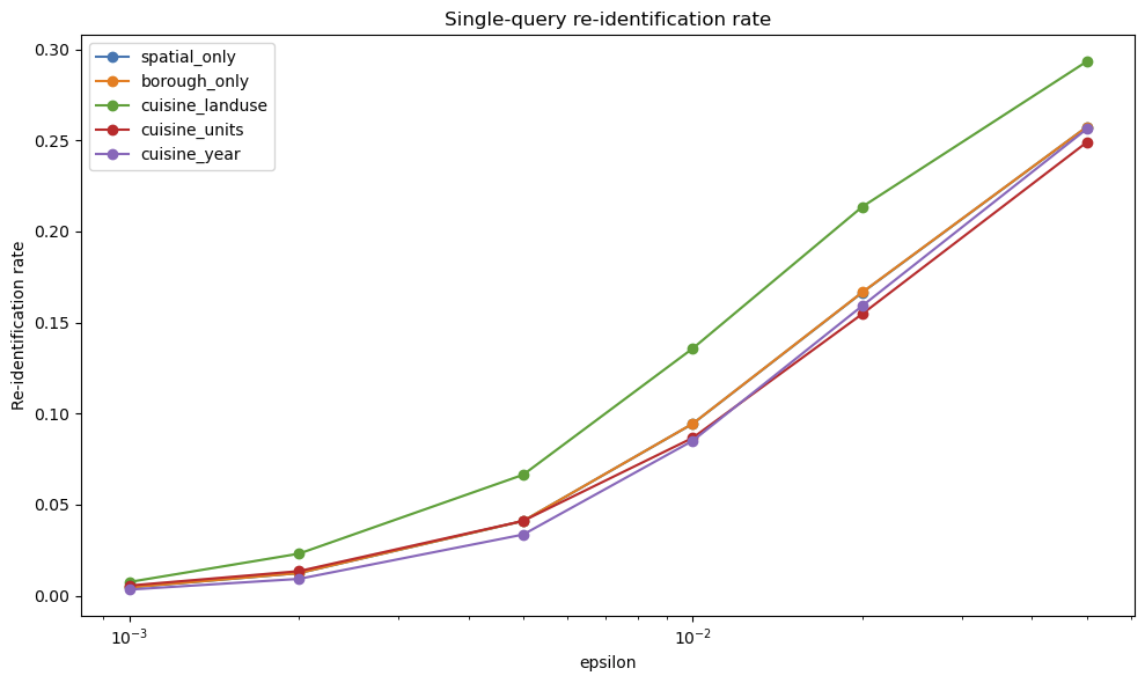
\includegraphics[width=0.8\textwidth]{fig_single_query.png}
    \caption{Single-query re-identification rate vs $\varepsilon$ for all prior configurations.}
    \label{fig:single_query}
\end{figure}

\subsection{Posterior analysis}

The theoretical bound from Theorem 3.1 is satisfied in 100\% of tested records and is conservative by approximately an order of magnitude. Median empirical posterior-to-prior ratios range from 2.3 to 3.8 across configurations, while the theoretical bounds for corresponding candidate set diameters are 100--1000x larger. Median attacker confidence at the true building $P(\text{true} \mid z)$ is 0.03\% at $\varepsilon = 0.001$ and 1.9\% at $\varepsilon = 0.01$. Fewer than 2\% of records have $P(\text{true} \mid z) > 0.5$ even at the weakest privacy setting. This means that the attacker's beliefs change very little after the supplementary data.

The strongest predictor of record-level vulnerability is the magnitude of the noise draw. Across all 200 combinations of attack configuration, $\varepsilon$, and cuisine type tested, the Spearman correlation between noise displacement and posterior-to-prior ratio ranges from $-0.89$ to $-0.96$ (all $p \approx 0$). Candidate count, borough, and cuisine type show no significant correlation. Privacy risk is fundamentally stochastic and is caused by a small fraction of records receiving insufficient noise by chance. These are the records an attacker can re-identify regardless of context.

\subsection{Multi-record attack}

Releasing a linkable identifier (CAMIS) measurably degrades privacy, but the degradation is less severe than the theoretical $n \cdot \varepsilon$ bound predicts. For spatial-only at $\varepsilon = 0.01$: $n = 1$ gives 9.45\%, $n = 2$ gives 11.5\%, $n = 3$ gives 15.2\%, $n = 4$ gives 15.8\%. With cuisine $\to$ landuse: $n = 1$ gives 13.6\%, $n = 3$ gives 20.0\%. The gains plateau around $n = 3$--$4$.

To test the composition bound, we compare multi-record re-identification to single-query at equivalent effective $\varepsilon$. For spatial-only: $n = 2$ at $\varepsilon = 0.005$ (effective $\varepsilon = 0.01$) achieves 4.7\%, compared to 9.45\% for a single query at $\varepsilon = 0.01$. The multi-record attack achieves substantially less than the theoretical worst case. The intersection constraint, which requires candidates to be spatially consistent across all observations, provides additional protection the bound does not account for.

The practical policy implication: at $\varepsilon = 0.01$, releasing CAMIS costs approximately 6 percentage points of additional re-identification risk (from 13.6\% to 20.0\% with 3 linked observations under the strongest prior). A data publisher can weigh this cost against the analytical benefit of tracking inspection histories.

\begin{figure}[H]
    \centering
    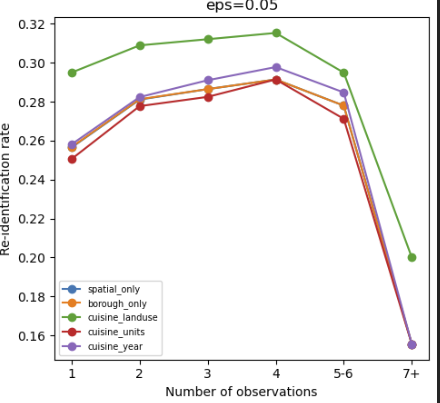
\includegraphics[width=0.55\textwidth]{fig_multi_record.png}
    \caption{Multi-record attack: re-identification rate vs number of observations.}
    \label{fig:multi_record}
\end{figure}

\subsection{Utility loss}

The mechanism introduces substantial analytical distortion at privacy levels where re-identification risk remains moderate. At $\varepsilon = 0.01$, cuisine composition TVD is 0.33 (a third of each tract's cuisine distribution changes) and inspection score RMSE is 8.08 points. At $\varepsilon = 0.001$, TVD rises to 0.60 and RMSE to 11.25. Data publishers face a quantifiable tradeoff: at $\varepsilon = 0.01$, the mechanism protects 86\% of restaurants against the strongest attack while introducing mean cuisine distortion of 0.33 TVD per tract.

\begin{figure}[H]
    \centering
    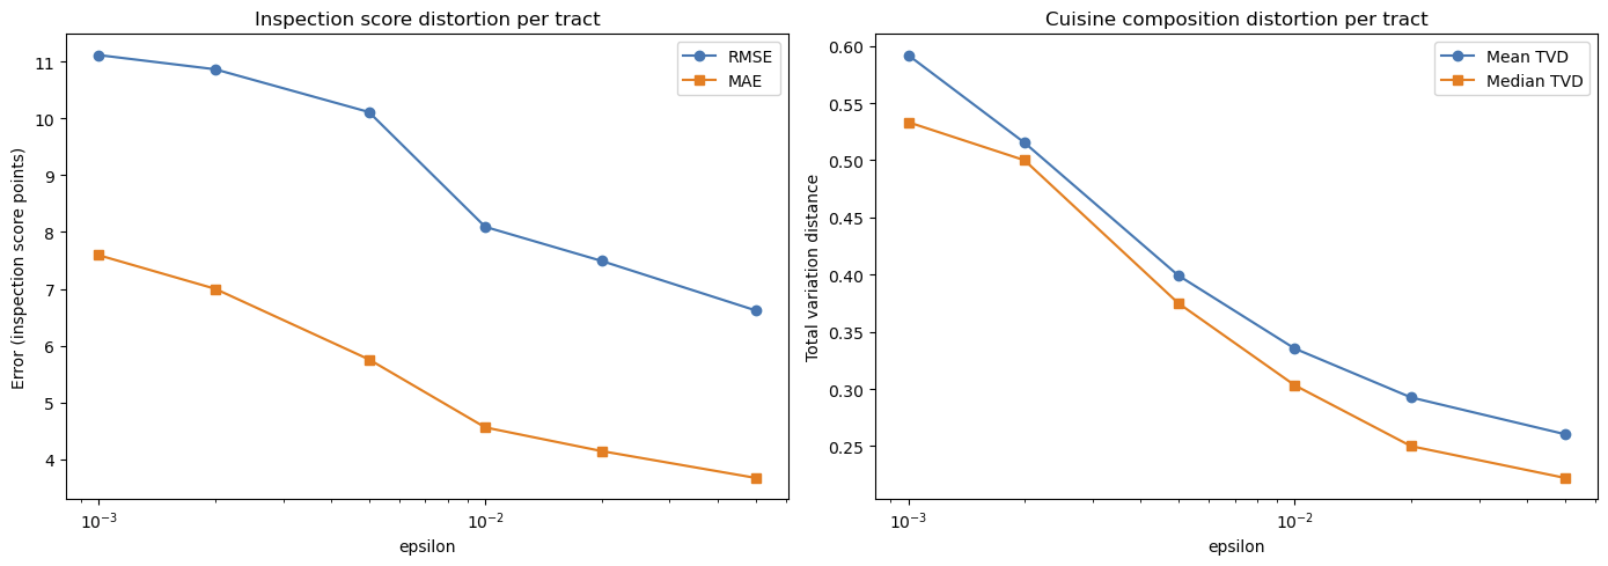
\includegraphics[width=0.8\textwidth]{fig_utility.png}
    \caption{Utility loss vs $\varepsilon$. Left: inspection score distortion (RMSE/MAE). Right: cuisine composition distortion (TVD).}
    \label{fig:utility}
\end{figure}

\begin{figure}[H]
    \centering
    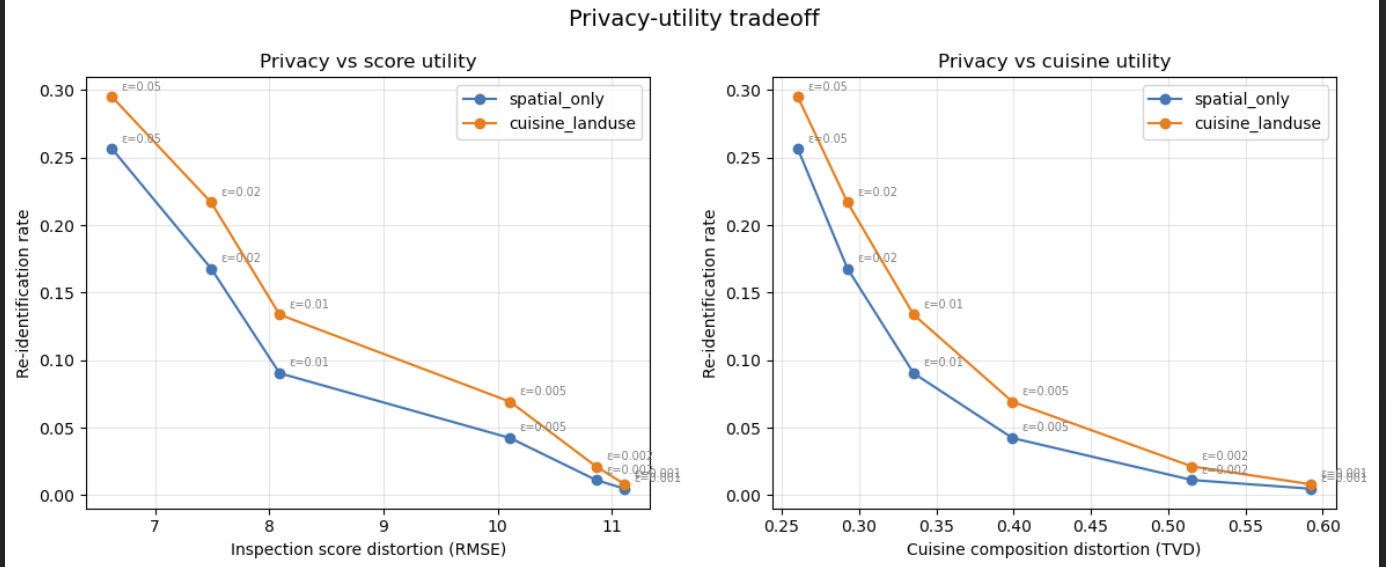
\includegraphics[width=0.8\textwidth]{fig_tradeoff.png}
    \caption{Privacy-utility tradeoff. Re-identification rate plotted against utility distortion for spatial-only and cuisine $\to$ landuse priors.}
    \label{fig:tradeoff}
\end{figure}

\section{Discussion}

The key insight is that the mechanism's effectiveness depends less on the attacker's auxiliary information and more on the stochastic noise draw, which the mechanism's design already accounts for. Each of our three metrics supports this from a different angle.

Re-identification rates show that even the strongest prior (cuisine $\to$ landuse) yields at most 4.7 percentage points of absolute improvement over spatial-only matching. The relative value of priors diminishes as $\varepsilon$ increases, from 86\% lift at $\varepsilon = 0.002$ to 14\% at $\varepsilon = 0.05$. This indicates that spatial proximity, not auxiliary knowledge, is the primary driver of attack success.

The posterior analysis confirms that the theoretical bound from Theorem 3.1 is conservative by an order of magnitude across all tested records. The near-perfect correlation between noise displacement and posterior-to-prior ratio ($\rho = -0.92$) means that vulnerability is determined by the random noise draw, not by which restaurant or which prior is used. This is reassuring for data publishers: no systematic class of records is disproportionately exposed.

The multi-record attack shows that the composition bound $n \cdot \varepsilon$ similarly overestimates empirical degradation. The spatial intersection constraint provides protection the worst-case theory does not capture, and gains plateau after 3--4 observations.

At the same time, utility loss is substantial. Even at $\varepsilon = 0.01$, cuisine composition distortion (TVD = 0.33) would meaningfully affect tract-level food access analyses. Publishers should select $\varepsilon$ based on the specific downstream analyses they need to preserve, using the privacy-utility curves this methodology produces.

The utility metric is the most customizable and will heavily influence the optimal epsilon value for a given dataset.

\textbf{Limitations.} This evaluation is specific to NYC's dense urban environment and may not generalize to suburban or rural settings where candidate density is lower. The smoothing parameter (0.01) in prior construction affects the balance between prior and spatial likelihood. The independence assumption when combining priors is violated in practice, which is why we test each individually. We evaluate a single mechanism (planar Laplace) and do not compare against alternatives such as deterministic rounding or the exponential mechanism. We also limited candidate sets to reduce computational costs (restricted radius and intersection requirement in multi-query attacks), so removing these restrictions could yield higher attack success.

\textbf{Future work.} Natural extensions include spatially adaptive $\varepsilon$ calibrated to local candidate density, posterior confidence ($P(\text{true} \mid z) > \text{threshold}$) as a stricter privacy metric, extension to non-Euclidean metric spaces ($d_X$-privacy, Chatzikokolakis et al., 2013), and a one-to-one bipartite matching attack enforcing the constraint that each building can only be matched once.

\section{References}

\noindent Andr\'es, M.~E., Bordenabe, N.~E., Chatzikokolakis, K., \& Palamidessi, C. (2013). Geo-indistinguishability: Differential privacy for location-based systems. \textit{CCS~'13}.

\noindent Chatzikokolakis, K., Andr\'es, M.~E., Bordenabe, N.~E., \& Palamidessi, C. (2013). Broadening the scope of differential privacy using metrics. \textit{PETS}.

\noindent Dwork, C., McSherry, F., Nissim, K., \& Smith, A. (2006). Calibrating noise to sensitivity in private data analysis. \textit{TCC}.

\noindent Reiter, J.~P. (2005). Estimating risks of identification disclosure in microdata. \textit{JASA}, 100(472), 1103--1112.

\noindent Sweeney, L. (2002). $k$-anonymity: A model for protecting privacy. \textit{IJUFKS}, 10(5), 557--570.

\end{document}
